\documentclass{bmstu}
% \usepackage[utf8]{inputenc}
% \usepackage{babel}
% \usepackage{listings}
% \usepackage{xcolor}

% \documentclass{article}
\usepackage[utf8]{inputenc}  % Кодировка входных данных
\usepackage[T2A]{fontenc}    % Шрифты для кириллицы
\usepackage{babel}  % Для поддержки русского языка
\usepackage{listings}        % Для вывода листингов
\usepackage{xcolor}

\lstset{ 
  backgroundcolor=\color{lightgray},   % Цвет фона
  basicstyle=\ttfamily\small,            % Шрифт и размер
  keywordstyle=\color{blue},              % Цвет ключевых слов
  commentstyle=\color{green},            % Цвет комментариев
  stringstyle=\color{red},               % Цвет строк
  numbers=left,                          % Номера строк слева
  numberstyle=\tiny\color{gray},         % Стиль номеров строк
  stepnumber=1,                          % Шаг номеров строк
  numbersep=5pt,                         % Расстояние между кодом и номерами строк
  showstringspaces=false,                % Не показывать пробелы в строках
  tabsize=2,                             % Размер табуляции
  breaklines=true,                       % Перенос строк
  breakatwhitespace=true,                % Переносить строки по пробелам
  captionpos=b,                          % Позиция заголовка
  frame=single,                          % Рамка вокруг кода
}

\begin{document}

% \makehomeworktitle
% \makeresearchtitle
\makereporttitle
{Информатика и системы управления (ИУ)}
{Программное обеспечение ЭВМ и информационные технологии (ИУ7)}
{Домашнему заданию}
{Программирование параллельных процессов}
{Распараллеливание с помощью MPI и OpenMP}
{16}
{Агарков~М.~В./ИУ7-32М}
% {М.В. Агарков}
{А.П. Ковтушенко}

\setcounter{page}{2}
\renewcommand{\contentsname}{Содержание} 
\tableofcontents

\chapter{Основная часть}

\section{Задание}

Разработать программу вычисления матрицы обратной заданной на основе метода Жордана.

Обосновать проектное решение (выбор алгоритма).
Обеспечить равномерную загрузку процессоров.
Результат вывести в тексовый файл.
Исследовать зависимость времени счета от размерности задачи и количества процессоров.

\section{Используемые формулы}

% Временная сложность алгоритма:
% \begin{equation}
%     T_{seq}(M) = O(M^3),
% \end{equation}
% где $M$ -- размерность матрицы.

Ускорение вычислений $S$:
\begin{equation}
    \label{eq:eq_s}
    S(M, N) = \frac{\mathit{Time}(M, 1)}{\mathit{Time}(M, N)},
\end{equation}
где $M$ -- размерность матрицы, $N$ -- количество вычислительных узлов.

Коэффициент эффективности $E$:
\begin{equation}
    \label{eq:eq_e}
    E(M, N) = \frac{S(M, N)}{N},
\end{equation}
где $M$ -- размерность матрицы, $N$ -- количество вычислительных узлов.


\section{Замеры времени}

\clearpage
Результаты замеров и вычислений с использованием MPI представлены в таблице 1.1:

\begin{table}[H]
    \center
    \caption{Результаты вычислений с использованием MPI}
    \label{tab:results-mpi}
    \fontsize{11pt}{11pt}\selectfont
    \begin{tabular}{|l|l|r|r|r|r|r|r|}
        \hline
        Размер & Кол-во процессов & 1 & 2 & 4 & 6 & 8 & 10 \\
        \hline
        % \multirow[t]{3}{*}{500}
        \multirow{500}
        & Эффективность (E) & 1.000 & 0.931 & 0.730 & 0.581 & 0.417 & 0.334 \\
        & Ускорение (S) &1.000 & 1.862 & 2.919 & 3.488 & 3.337 & 3.344 \\
        & Время &0.635 & 0.341 & 0.217 & 0.182 & 0.190 & 0.189 \\
        \cline{1-8}
        % \multirow[t]{3}{*}{1000}
        \multirow{1000}
        & Эффективность (E) & 1.000 & 0.966 & 0.815 & 0.724 & 0.633 & 0.591 \\
        & Ускорение (S) &1.000 & 1.932 & 3.261 & 4.347 & 5.068 & 5.913 \\
        & Время &5.140 & 2.661 & 1.576 & 1.182 & 1.014 & 0.869 \\
        \cline{1-8}
        % \multirow[t]{3}{*}{1500}
        \multirow{1500}
        & Эффективность (E) & 1.000 & 0.986 & 0.907 & 0.840 & 0.746 & 0.673 \\
        & Ускорение (S) &1.000 & 1.972 & 3.629 & 5.040 & 5.974 & 6.738 \\
        & Время &17.515 & 8.880 & 4.827 & 3.476 & 2.931 & 2.599 \\
        \cline{1-8}
        % \multirow[t]{3}{*}{2000}
        \multirow{2000}
        & Эффективность (E) & 1.000 & 0.981 & 0.938 & 0.875 & 0.768 & 0.752 \\
        & Ускорение (S) &1.000 & 1.962 & 3.755 & 5.255 & 6.150 & 7.520 \\
        & Время &41.489 & 21.145 & 11.048 & 7.895 & 6.746 & 5.517 \\
        \cline{1-8}
        % \multirow[t]{3}{*}{2500}
        \multirow{2500}
        & Эффективность (E) & 1.000 & 0.998 & 0.943 & 0.901 & 0.812 & 0.753 \\
        & Ускорение (S) &1.000 & 1.996 & 3.772 & 5.408 & 6.498 & 7.535 \\
        & Время &81.145 & 40.643 & 21.513 & 15.005 & 12.487 & 10.772 \\
        \cline{1-8}
        % \multirow[t]{3}{*}{3000}
        \multirow{3000}
        & Эффективность (E) & 1.000 & 0.995 & 0.951 & 0.923 & 0.799 & 0.762 \\
        & Ускорение (S) &1.000 & 1.991 & 3.805 & 5.538 & 6.392 & 7.629 \\
        & Время &139.181 & 69.917 & 36.581 & 25.133 & 21.770 & 18.242 \\
        \cline{1-8}
    \end{tabular}
\end{table}


Результаты замеров и вычислений с использованием OpenMP представлены в таблице 1.2:

\begin{table}[H]
    \center
    \caption{Результаты вычислений с использованием OpenMP}
    \label{tab:results-openmp}
    \fontsize{11pt}{11pt}\selectfont
    \begin{tabular}{|l|l|r|r|r|r|r|r|}
        \hline
        Размер & Кол-во процессов & 1 & 2 & 4 & 6 & 8 & 10 \\
        \hline
        % \multirow[t]{3}{*}{500}
        \multirow{500}
        & Эффективность (E) & 1.000 & 0.902 & 0.435 & 0.304 & 0.202 & 0.156 \\
        & Ускорение (S) &1.000 & 1.803 & 1.738 & 1.824 & 1.617 & 1.560 \\
        & Время &0.244 & 0.135 & 0.140 & 0.133 & 0.151 & 0.156 \\
        \cline{1-8}
        % \multirow[t]{3}{*}{1000}
        \multirow{1000}
        & Эффективность (E) & 1.000 & 0.967 & 0.639 & 0.468 & 0.369 & 0.337 \\
        & Ускорение (S) &1.000 & 1.933 & 2.556 & 2.810 & 2.949 & 3.372 \\
        & Время &1.706 & 0.882 & 0.667 & 0.607 & 0.578 & 0.506 \\
        \cline{1-8}
        % \multirow[t]{3}{*}{1500}
        \multirow{1500}
        & Эффективность (E) & 1.000 & 0.866 & 0.618 & 0.605 & 0.516 & 0.495 \\
        & Ускорение (S) &1.000 & 1.732 & 2.472 & 3.628 & 4.127 & 4.945 \\
        & Время &5.813 & 3.355 & 2.352 & 1.602 & 1.409 & 1.175 \\
        \cline{1-8}
        % \multirow[t]{3}{*}{2000}
        \multirow{2000}
        & Эффективность (E) & 1.000 & 0.999 & 0.752 & 0.682 & 0.608 & 0.537 \\
        & Ускорение (S) &1.000 & 1.999 & 3.058 & 4.091 & 4.865 & 5.373 \\
        & Время &13.966 & 6.986 & 4.641 & 3.414 & 2.870 & 2.599 \\
        \cline{1-8}
        % \multirow[t]{3}{*}{2500}
        \multirow{2500}
        & Эффективность (E) & 1.000 & 0.954 & 0.739 & 0.689 & 0.610 & 0.605 \\
        & Ускорение (S) &1.000 & 1.908 & 2.956 & 4.131 & 4.877 & 6.046 \\
        & Время &25.988 & 13.622 & 8.792 & 6.292 & 5.329 & 4.299 \\
        \cline{1-8}
        % \multirow[t]{3}{*}{3000}
        \multirow{3000}
        & Эффективность (E) & 1.000 & 0.981 & 0.839 & 0.728 & 0.658 & 0.628 \\
        & Ускорение (S) &1.000 & 1.961 & 3.355 & 4.368 & 5.262 & 6.276 \\
        & Время &44.663 & 22.773 & 13.310 & 10.224 & 8.488 & 7.115 \\
        \cline{1-8}
    \end{tabular}
\end{table}



\section{Построение графиков}

Результаты сравнения программ приведены на рисунках 1.1 - 1.6:


\begin{figure}[H]
    \centering
		{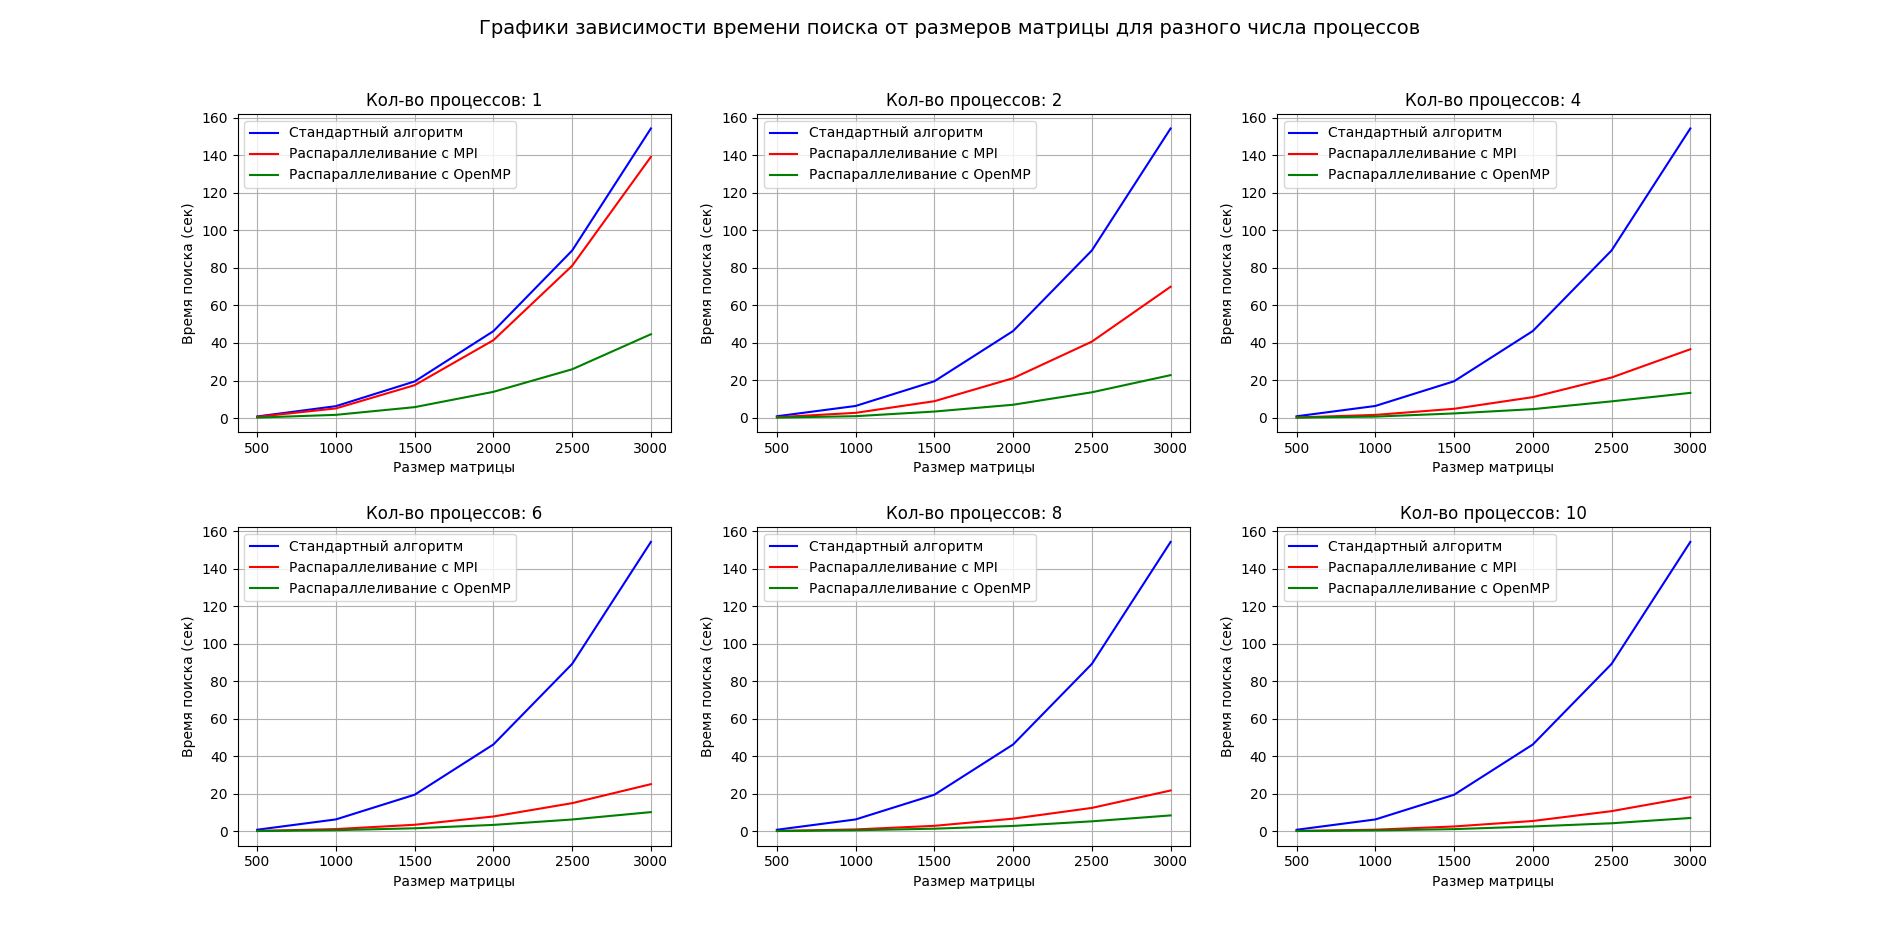
\includegraphics[scale = 0.29, angle=0]{../img/comp_thread_count.png}}
		\caption{Графики зависимости времени поиска от размеров матрицы для разного числа процессов}
		\label{fig:compare_thread_count}
	% \end{center}
\end{figure}


\begin{figure}[H]
	\begin{center}
		{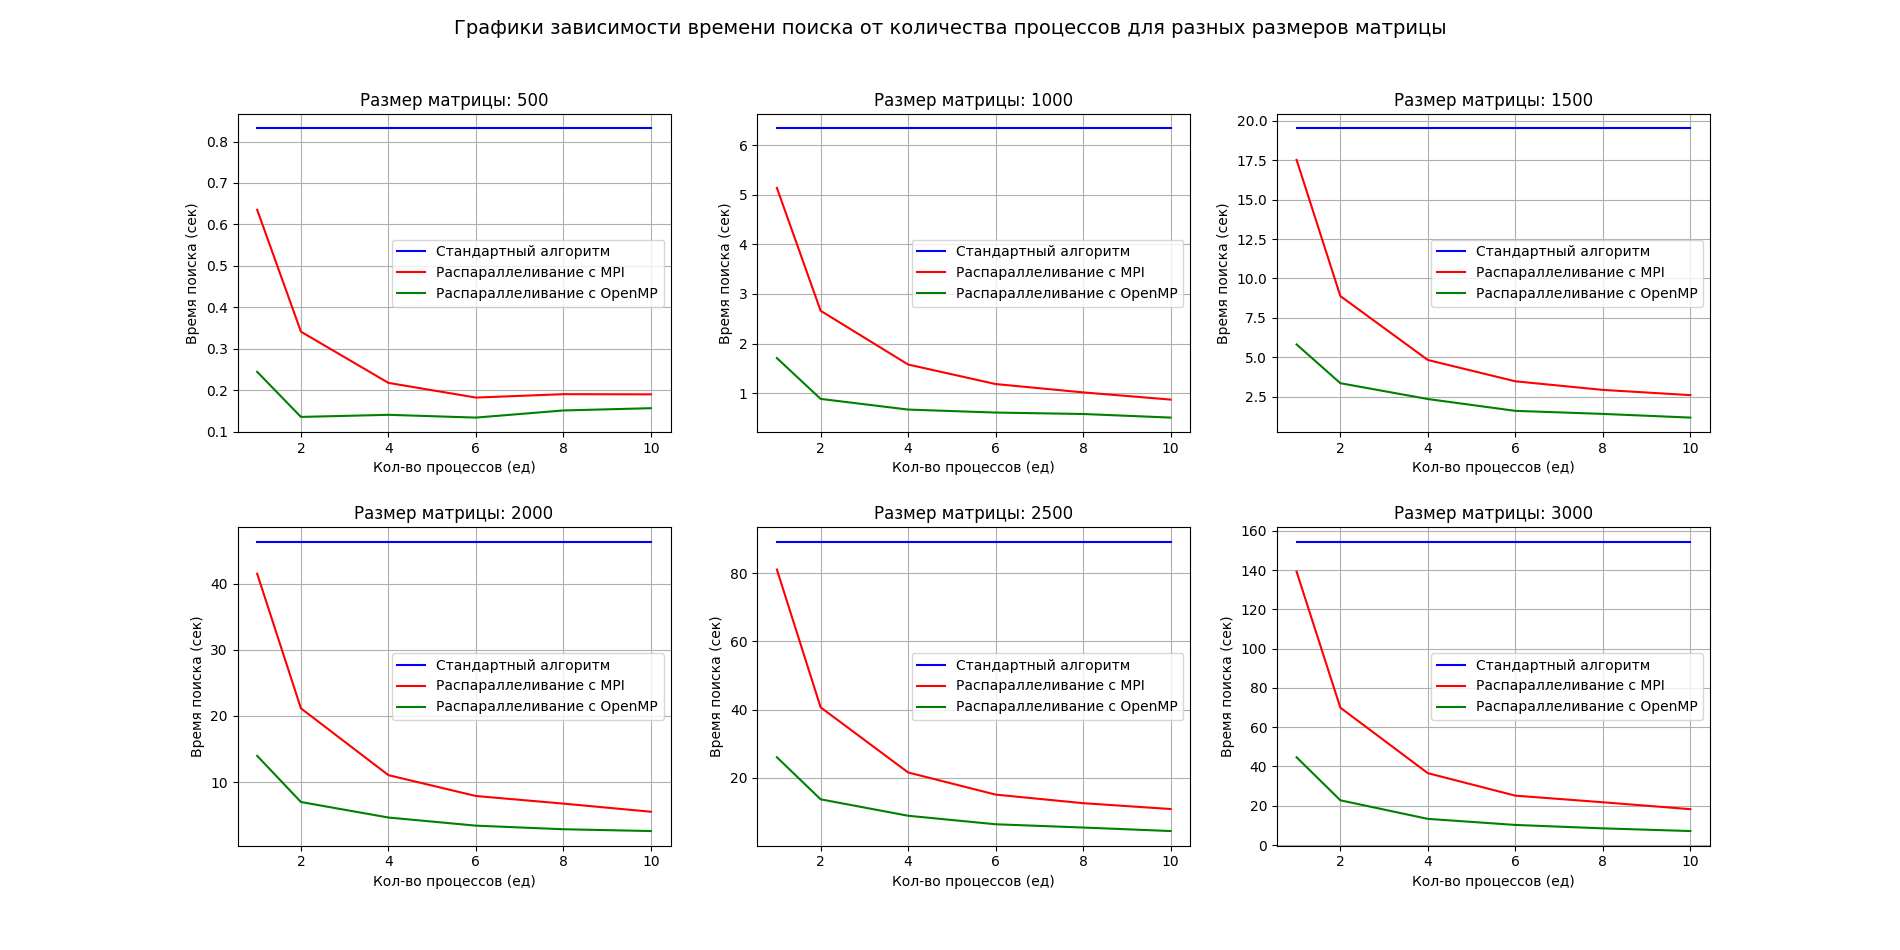
\includegraphics[scale = 0.29, angle=0]{../img/comp_size_matrix.png}}
		\caption{Графики зависимости времени поиска от количества процессов для разных размеров матрицы}
		\label{fig:compare_size_matrix}
	\end{center}
\end{figure}


\begin{figure}[H]
	\begin{center}
		{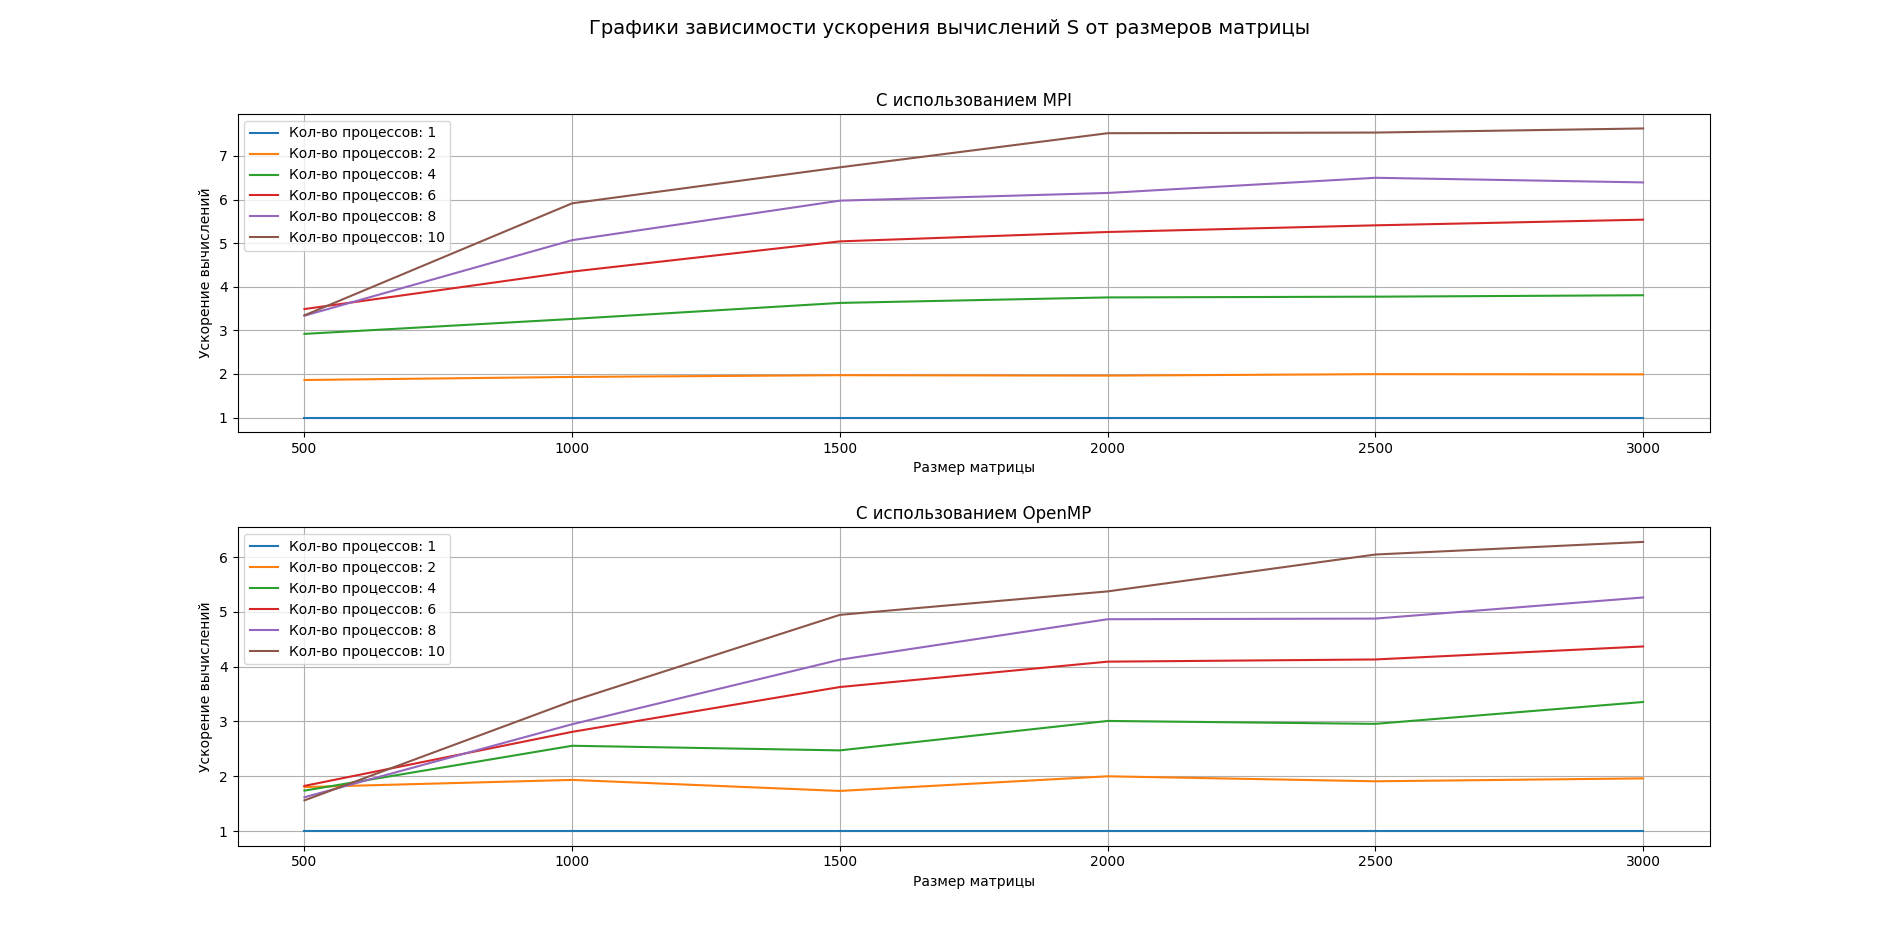
\includegraphics[scale = 0.29, angle=0]{../img/comp_speed_up_matrix_size.png}}
		\caption{Графики зависимости ускорения вычислений S от размера матрицы}
		\label{fig:compare_speed_up_matrix_size}
	\end{center}
\end{figure}


\begin{figure}[H]
	\begin{center}
		{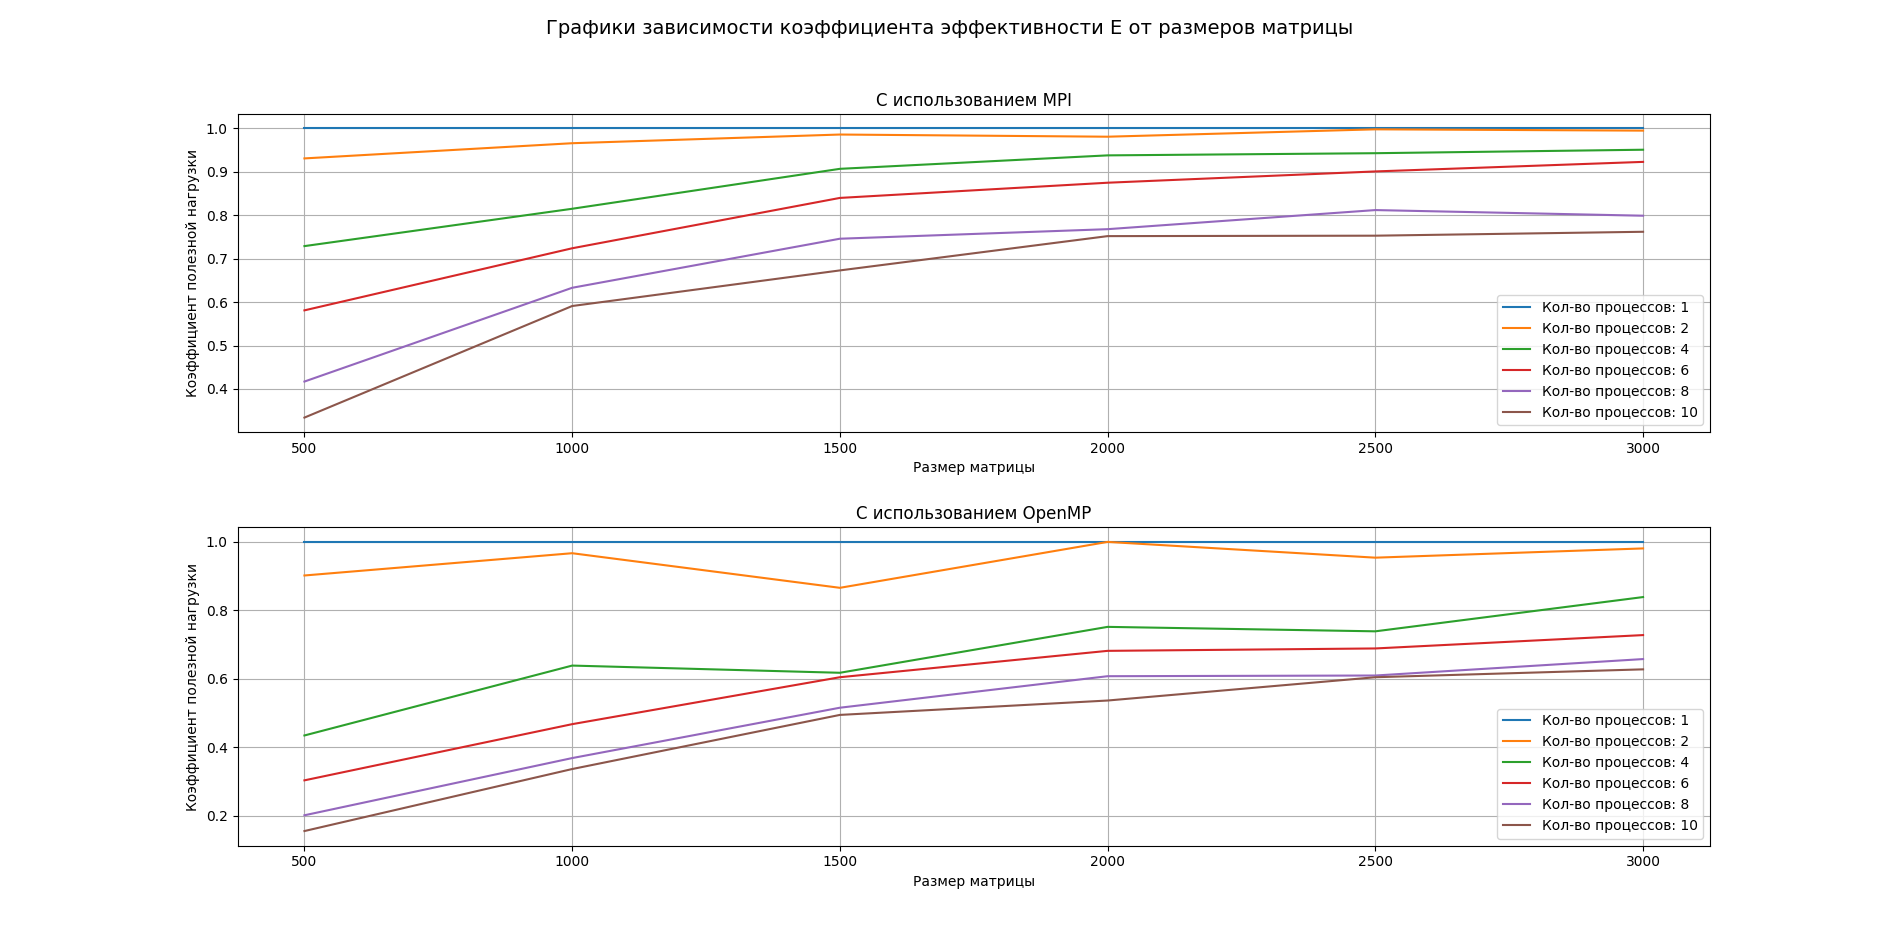
\includegraphics[scale = 0.29, angle=0]{../img/comp_efficiency_on_matrix_size.png}}
		\caption{Графики зависимости коэффициента эффективности E от размера матрицы}
		\label{fig:compare_efficiency_matrix_size}
	\end{center}
\end{figure}


\begin{figure}[H]
	\begin{center}
		{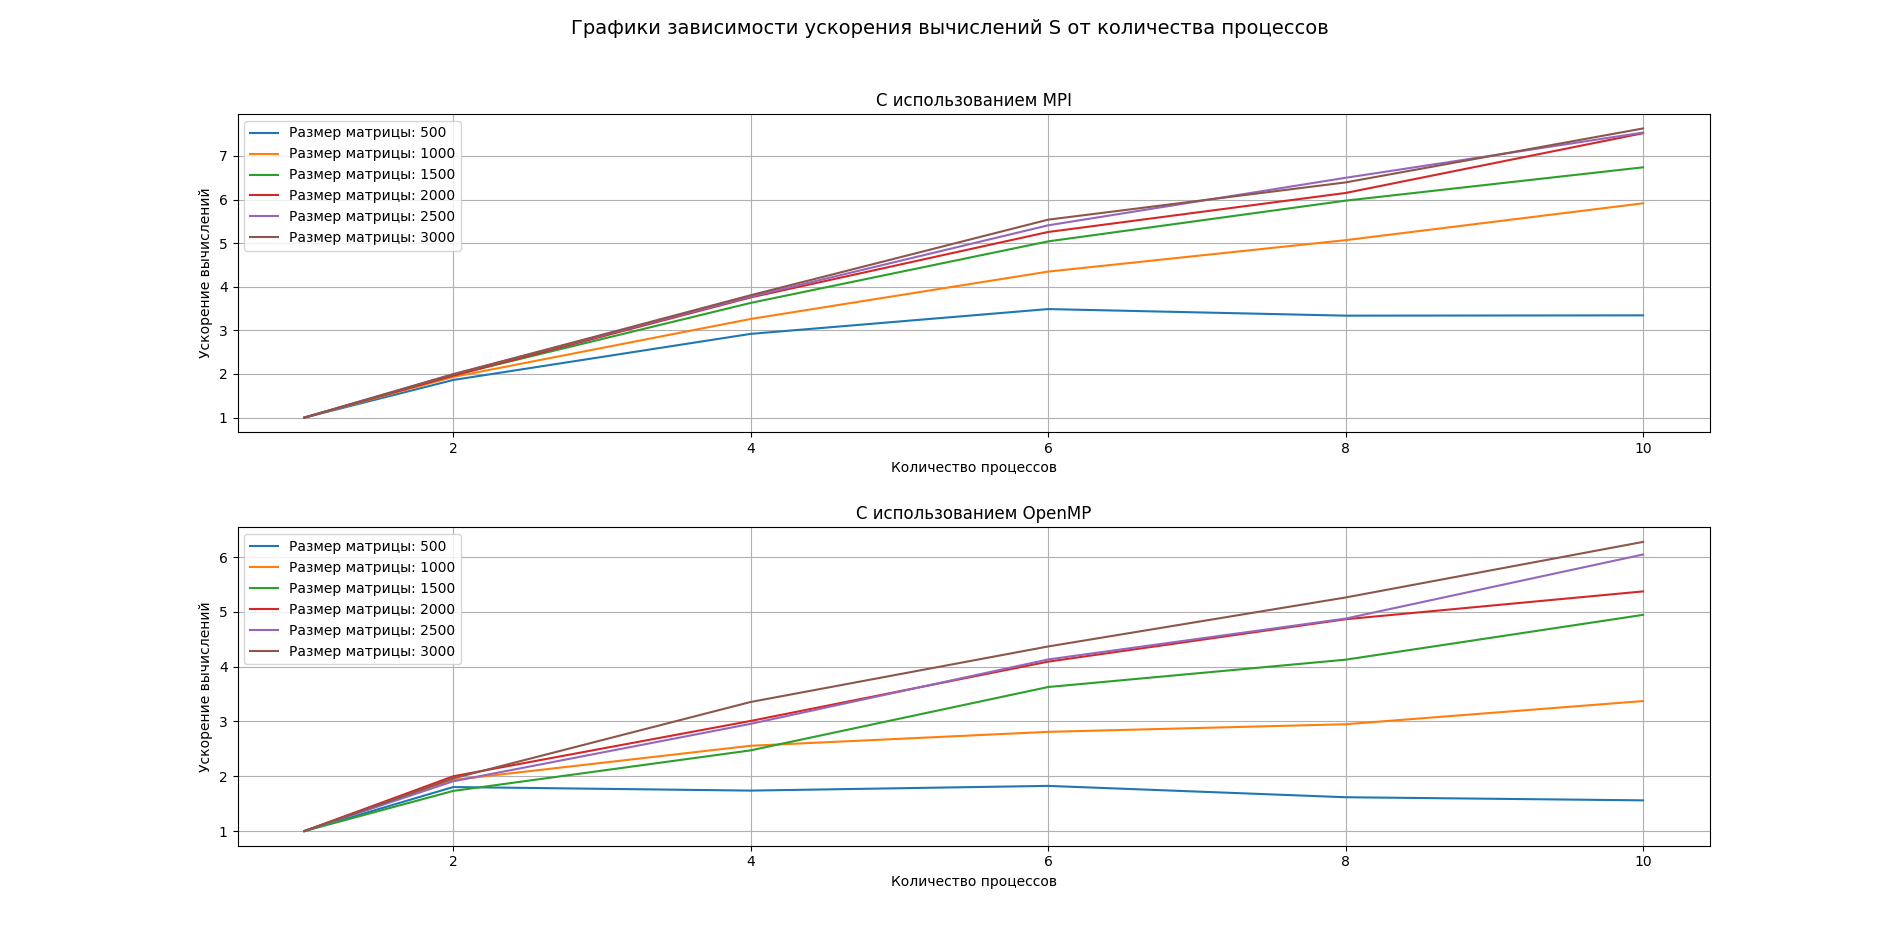
\includegraphics[scale = 0.29, angle=0]{../img/comp_speed_up_threads_count.png}}
		\caption{Графики зависимости ускорения вычислений S от количества процессов}
		\label{fig:compare_speed_up_threads_count}
	\end{center}
\end{figure}


\begin{figure}[H]
	\begin{center}
		{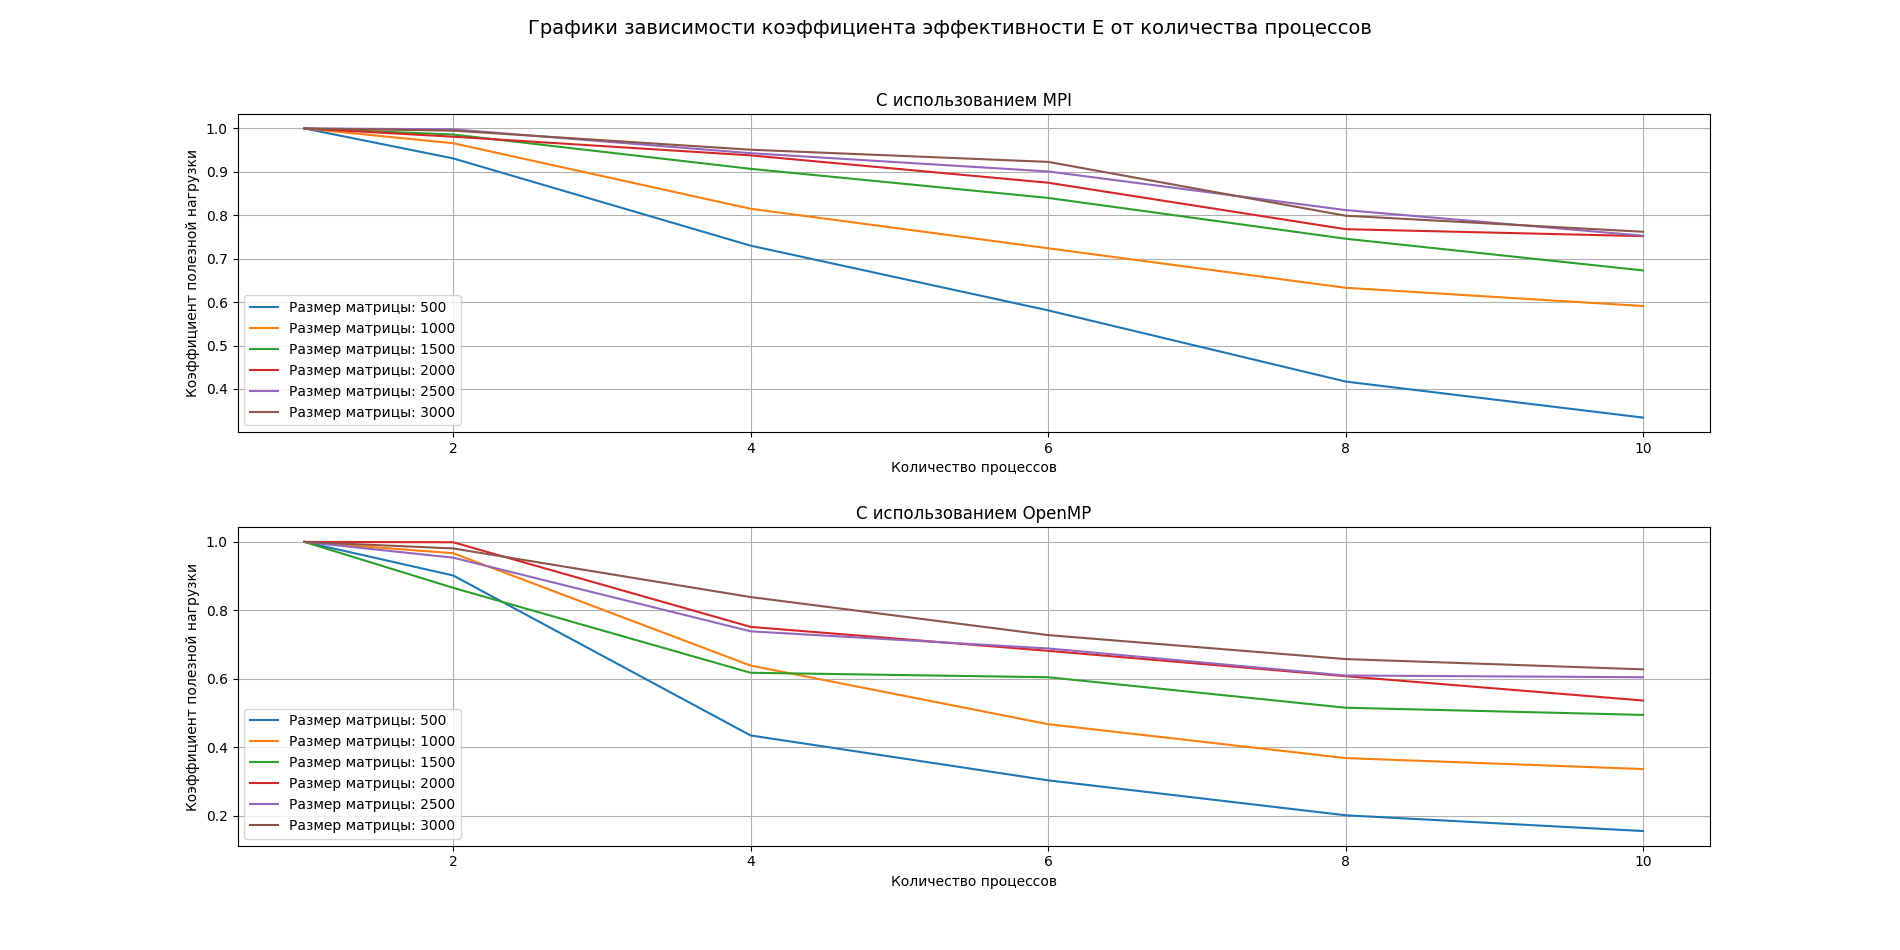
\includegraphics[scale = 0.29, angle=0]{../img/comp_efficiency_on_threads_count.png}}
		\caption{Графики зависимости коэффициента эффективности E от количества процессов}
		\label{fig:compare_efficiency_threads_count}
	\end{center}
\end{figure}


\end{document}